\documentclass[11pt]{article}

\usepackage{thumbpdf, amssymb, amsmath, amsthm, microtype,
	    graphicx, verbatim, listings, color, fancybox}
\usepackage[pdftex]{hyperref}
%\usepackage[margin=1in]{geometry}
\usepackage{cawsty}
\usepackage{fullpage}
\usepackage{pseudocode}
\usepackage{verbatim}
\usepackage{multicol}

\usepackage{fancybox}
\usepackage{tikz}

\newcommand{\tlg}{\text{lg}}
\newcommand{\tln}{\text{ln}}
\newcommand{\tlog}{\text{log}}

\usepackage{algorithm}
%\usepackage{algorithmic}
\usepackage{amsmath}
\usepackage{amsthm}
\usepackage{algpseudocode}
\usepackage{algorithmicx}% http://ctan.org/pkg/algorithmicx
\usepackage{lipsum}% http://ctan.org/pkg/lipsum
\usepackage{xifthen}% http://ctan.org/pkg/xifthen
\usepackage{needspace}% http://ctan.org/pkg/needspace
\usepackage{hyperref}% http://ctan.org/pkg/hyperref

\usepackage{tikz}
\usetikzlibrary{arrows,%
                shapes,positioning}

\tikzstyle{vertex}=[circle,fill=black!25,minimum size=20pt,inner sep=0pt]
\tikzstyle{selected vertex} = [vertex, fill=red!24]
\tikzstyle{edge} = [draw,thick,-]
\tikzstyle{weight} = [font=\small]
\tikzstyle{selected edge} = [draw,line width=5pt,-,red!50]
\tikzstyle{ignored edge} = [draw,line width=5pt,-,black!20]

\allowdisplaybreaks[1]

% ================ ALGORITHM ENVIRONMENT ================
\newcounter{numberedAlg}% Algorithm counter
\newenvironment{numberedAlg}[1][]%
  {% \begin{numberedAlg}[#1]
    \needspace{2\baselineskip}% At least 2\baselineskip required, otherwise break
    \noindent \rule{\linewidth}{1pt} \endgraf% Top rule
    \refstepcounter{numberedAlg}% For correct reference of algorithm
    \centering \textsc{Algorithm}~\thenumberedAlg%
    \ifthenelse{\isempty{#1}}{}{:\ #1}% Typeset name (if provided)
  }{% \end{numberedAlg}
  \noindent \rule{\linewidth}{1pt}% Bottom rule
  }%

%\setlength{\parindent}{0pt}

\linespread{1.2}

\begin{document}
\cawtitle{4005-800 Algorithms}{Homework 7}

\begin{prob}{1 - 34.2-1}
Consider the language GRAPH-ISOMORPHISM = $\{\langle G_1, G_2 \rangle : G_1$ and $G_2$ are isomorphic graphs $\}$. Prove that GRAPH-ISOMORPHISM $\in NP$ by describing a polynomial-time algorithm to verify the language.
\end{prob}
\begin{sol}
By the defintion of graph isomorphism, two graphs $G_1$ and $G_2$ are isomorphic if and only if there exists a bijection $m : V(G_1) \to V(G_2)$ such that any two vertices $v_i$ and $v_j$ of $G_1$ are adjacent in $G_1$ if and only if $m(v_i)$ and $m(v_j)$ are adjacent in $G_2$. With this definition, it is enough to check the bijection $m$ to see if it fulfills this property to verify that two graphs isomorphic. We can easily devise a polynomial-time algorithm to solve this as follows:

\begin{numberedAlg}[GRAPH-ISOMORPHISM-VERIFIER]
\label{alg1}
\begin{algorithmic}[1]
	\Function{VerifyGraphIsomorphism}{$m$}
		\ForAll{$v_{i} \in V(G_1)$}
			\State vCount = 0 \Comment {Count number of times $v_i$ appears in $G_2$}
			\ForAll{$v_j \in V(G_2)$}
				\If{$m(v_i) == v_j$}
					\State vCount = vCount + 1
				\EndIf
			\EndFor
			\If {vCount $\not= 1$} \Comment {$v_i$ should only appear once in $G_2$}
				\State \Return False
			\EndIf
		\EndFor
\\
		\ForAll{$v_i \in V(G_1)$}
			\ForAll{$v_j \in V(G_1)$}
				\If{$(v_i, v_j) \in E(G_1)$ and $(m(v_i), m(v_j)) \notin E(G_2)$}
					\State \Return False
				\EndIf
			\EndFor
		\EndFor
\\
		\ForAll{$v_i \in V(G_1)$}
			\ForAll{$v_j \in V(G_1)$}
				\If{$(m(v_i), m(v_j)) \in E(G_2)$ and $(v_i, v_j) \notin E(G_1)$}
					\State \Return False
				\EndIf
			\EndFor
		\EndFor
\\
		\State \Return True
	\EndFunction
\end{algorithmic}
\end{numberedAlg}

Note that $m$ denotes the bijective mapping (the permutation) from $V(G_1)$ to $V(G_2)$. It is clear that the permutation check runs in $O(V)$ time and the edge check runs in $O(V^2)$ time. Thus, we conclude that this algorithms runs in $O(V^2)$ time and thus verifies the solution (i.e. the permutation mapping $m$) to the GRAPH-ISOMORPHISM problem in polynomial time. 
\end{sol}

\begin{prob}{2 - 34.2-10}
Prove that if $NP \not= co$-$NP$, then $P \not= NP$.
\end{prob}
\begin{sol}
If $NP \not= co$-$NP$, then we know there exists a problem $Q \in NP$ such that $Q \notin co$-$NP$.  Furthermore, by definition, we know that $P \in co$-$NP \cap NP$. Now, let $Q$ be a problem in $NP$ that is not in $co$-$NP$. By the definition of the set intersection, that means that $Q \notin co$-$NP \cap NP$, and thus we know that $Q \in NP$ and $Q \notin P$ (becuse $P$ is a subset of $co$-$NP \cap NP$). Therefore, since there exists a problem that is in $NP$ but not in $P$, we conclude that $P \not= NP$. 
\end{sol}

\begin{prob}{3 - 34.3-1}
Verify that the circuit in Figure $34.8(b)$ is unsatisfiable.
\end{prob}
\begin{sol}
\begin{center}
	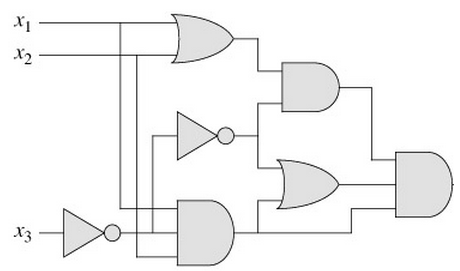
\includegraphics[scale=0.5]{circuit.png} \\
\end{center}

The logical equivalent expression for this circuit is as follows:
\begin{eqnarray*}
((x_1 \lor x_2) \land x_3) \land (x_3 \lor (x_1 \land x_2 \land \lnot x_3)) \land (x_1 \land x_2 \land \lnot x_3)
\end{eqnarray*}

To show that this circuit is unsatisfiable, we simply build a truth table for the boolean expression that considers all logical values for $x_1, x_2,$ and $x_3$, as shown in table \ref{thetable}:

\begin{table}
\centering
    \begin{tabular}{|l|l|l|l|l|l|}
        \hline
        $x_1, x_2, x_3$ & $x_1 \lor x_2$ & $(x_1 \lor x_2) \land x_3$ & $x_1 \land x_2 \land \lnot x_3$ & $x_3 \lor (x_1 \land x_2 \land \lnot x_3)$ & Final AND Gate \\ \hline
        F,F,F & F & F & F & F & F \\ 
        F,F,T & F & F & F & T & F \\ 
        F,T,F & T & F & F & F & F \\ 
        F,T,T & T & T & F & T & F \\ 
        T,F,F & T & F & F & F & F \\ 
        T,F,T & T & T & F & T & F \\ 
        T,T,F & T & F & T & T & F \\ 
        T,T,T & T & T & F & T & F \\ 
        \hline
    \end{tabular}
	\label{thetable}
	\caption{Truth table for problem \#3, where T = True and F = False.}
\end{table}

Therefore, since there is no possible combination of logical values for $x_1$, $x_2$, and $x_3$ such that the boolean expression is true, we conclude that it is unsatisfiable.

\end{sol}

\begin{prob}{4 - 34.4-5}
Show that the problem of determining the satisfiability of boolean formulas in disjunctive normal form is polynomial-time solvable.
\end{prob}
\begin{sol}
We show that the problem of determining the satisfiability of boolean formulas in disjunctive normal form is polynomial-time solvable by providing a polynomial-time algorithm that performs this task. This algorithm is realized below in Algorithm \ref{alg2}.

\begin{numberedAlg}[DNF-SOLVER]
\label{alg2}
\begin{algorithmic}[1]
	\Function{SolveDNF}{$\psi$}
		\ForAll{Logical clauses $c_i \in \psi$}
			\State $satisfiable = True$
			\State $satList = makeQueue()$
			\ForAll{Literals $l_j \in c_i$}
				\ForAll{Literals $l_k \in satList$}
					\If{$l_j == \lnot l_j$}
						\State $satisfiable$ = False \Comment{Found the negation of $l_j$ in the queue}
					\EndIf
				\EndFor
				\State $PUSH(satList, l_j)$ \Comment{Push this literal into the queue}
			\EndFor
			\If{$satisfiable == True$}
				\State \Return $True$
			\EndIf
		\EndFor
		\State \Return $False$
	\EndFunction
\end{algorithmic}
\end{numberedAlg}

Since DNF statements are composed of disjunctions (ORs) of conjunction clauses (ANDs), it is enough to check and see if only one conjunction clause can be satisfied. Therefore, this procedure simply traverses over every clause and checks to see if there is a literal and its negation in that clause, which indicates that the clause can never be true. If this is not the case, then the clause must be satisfiable, and thus the expression is satisfiable. 

The time complexity of this algorithm is $O(mn^2)$, where $m$ is the number of clauses in $\psi$ and $n$ is the number of literals in the boolean expression. The reason for this is that for every clause we traverse over every literal in the clause, and for each element we perform a linear search with $satList$ that can be equal to the number of literals in the clause. Therefore, since the linear search runs in $O(n)$ time, the number of literals in a clause is $O(n)$, and the number of clauses in $\psi$ is $O(m)$, and each of these operations are nested, the resulting time complexity is $O(mn^2)$.

\end{sol}

\begin{prob}{5 - 34.5-5}
The \textbf{set-partition problem} takes as input a set $S$ of numbers. The question is whether the numbers can be partitioned into two sets $A$ and $A' = S - A$ such that $\sum_{x \in A}x = \sum_{x \in A'} x$. Show that the set-partition problem is $NP$-complete.
\end{prob}
\begin{sol}
In order to show that the set-partition problem, $Q$ is $NP$-complete, we show that it reduces to the subset-sum problem, $Q'$. That is, we prove $Q \leq_p Q'$ as follows:
\begin{itemize}
	\item Given instance of left, build instance to right
	\item Show that right solves
	\item Show that construction solves left
	\item Show that construction can be done in polynomial time
\end{itemize}
\end{sol}

\begin{prob}{6-a}
Write pseudo-code for a recursive solution to the variation on the 0-1 knapsack problem that computes the
maximum value that can be placed in the knapsack.
\end{prob}
\begin{sol}
\begin{numberedAlg}[RECURSIVE 0-1 KNAPSACK]
\label{alg2}
\begin{algorithmic}[1]
	\Function{RecursiveKnapsack}{$n, v, w, W$}
		\If{$W < 0$}
			\State \Return $-1$ \Comment{The weight limit was passed, so decrease the value}
		\ElsIf{$n == 0$}
			\State \Return $0$ \Comment{There are no items to contribute weight or value}
		\Else
			\State \Return max($v[n]+RecursiveKnapsack(n-1, v, w, W-w[n])$, \\ $RecursiveKnapsack(n-1,v,w,W)$)
		\EndIf
	\EndFunction
\end{algorithmic}
\end{numberedAlg}
\end{sol}

\begin{prob}{6-b}
Give a dynamic programming solution to the 0-1 knapsack problem that is based on the previous problem;
this algorithm should return the items to be taken. Implement this algorithm and call it $knapsack$.
\end{prob}
\begin{sol}
TODO: insert source code once finished.
\end{sol}

\begin{prob}{6-c}
What is the time complexity of your dynamic programming based algorithm?
\end{prob}
\begin{sol}
The time complexity of this dynamic programming based algorithm depends on the computation of the $value$ table and identifying the items that were added to the knapsack. Since these procedures are run back-to-back, we consider their time complexity separately in order to determine the time complexity of the entire algorithm.

The time complexity of the value computation depends on the initialization procedure in which the table is constructed and then the nested loops that perform the bottom-up computation. The initialization procedure generates a table that has dimensions $n \times W$, so it runs in $O(nW)$ time. Similarly, the table computation procedure performs a constant time table lookup (or returns a $0$ in the base case) when traversing across every possible knapsack capacity for every item, so we can conclude that this procedure runs in $O(nW)$ time as well.

Analyzing the time complexity of the item identification procedure indicates that it runs in $O(n)$ time, because at every iteration through the main loop the item counter is decreased by $1$ until we consider all items in the knapsack. Hence, the linear time complexity of $O(n)$.

Now, putting these two results together, the dynamic programming based algorithm that solves the 0-1 knapsack problem has a time complexity of $O(nW) + O(nW) + O(n)$, which can be reduced to $O(nW)$. 
\end{sol}

\begin{prob}{6-d}
The knapsack decision problem is $NP$-complete. Does your analysis above prove that $P = NP$? Explain.
\end{prob}
\begin{sol}
TODO: no? it's just a fancy implementation...
\end{sol}

\end{document}
